\documentclass[12pt,notitlepage]{report}
%\pagestyle{headings}
\pagestyle{plain}

\usepackage[utf8]{inputenc} 
\usepackage{a4wide} 
%\usepackage{index} % nutno použít v případě tvorby rejstříku balíčkem makeindex
%\usepackage{fancybox} % umožňuje pokročilé rámečkování :-)
\usepackage{graphicx} % nezbytné pro standardní vkládání obrázků do dokumentu

\usepackage[twoside, inner=4cm, outer=3cm, top=3cm, bottom=3cm]{geometry} % nastavení dané velikosti okrajů
\usepackage{thesis}
\usepackage{hyperref}
\usepackage[round]{natbib}
\usepackage{multirow}
\usepackage{array}
\usepackage{listings}

% pro scenario soubory
\lstdefinelanguage{scenario}{
    morekeywords={task,algorithm,in,out,params,end},
    sensitive=true,
    morecomment=[l]{\#},
    morestring=[b]",
}
\lstset{
    language=scenario,
    basicstyle=\footnotesize,
    keywordstyle=\bf,
    showstringspaces=false,
    stringstyle=\color{red},
    commentstyle=\color{blue},
    escapechar=\^,
}

%\newindex{default}{idx}{ind}{Rejstřík} % zavádí rejstřík v případě použití balíku index
\usepackage{nomencl}
\makenomenclature
\renewcommand{\nomname}{List of Abbreviations}

\title{Deep Automatic Analysis of English}  
\def\fulldate{August 6th, 2010}
\author{Ondřej Dušek}
\date{2010}
\dept{Institute of Formal and Applied Linguistics}
\studyprogram{Computer Science}
\studyfield{Mathematical Linguistics}
\supervisor{Prof. RNDr. Jan Hajič, Dr.}

\begin{document}

\maketitle

\pagestyle{plain}
\normalsize % nastavení normální velikosti fontu
\setcounter{page}{2} % nastavení číslování stránek
\cleardoublepage
\ \vspace{10mm} 

\noindent % podekovani
 
\vspace{\fill}
\noindent I certify that this diploma thesis is my own work, and that only I used the cited literature. The thesis is freely available for all who can use it.

 
\bigskip
\noindent Prague, \fulldate \hspace{\fill}\theauthor\\ % doplňte patřičné datum, jméno a příjmení

%%%   Výtisk pak na tomto míste nezapomeňte PODEPSAT!
%%%                                         *********

\cleardoublepage
\tableofcontents % vkládá automaticky generovaný obsah dokumentu

\cleardoublepage % přechod na novou stránku
\pagestyle{plain}
\addcontentsline{toc}{chapter}{Abstract}
%%% Následuje strana s abstrakty. Doplňte vlastní údaje.
\noindent
Title: \thetitle\\
Author: \theauthor\\
Department: \thedept\\
Supervisor: \thesupervisor\\
Supervisor's e-mail address: \texttt{hajic@ufal.mff.cuni.cz}\\

\noindent Abstract: In the present work we study ... Uvede se anglický abstrakt v rozsahu 80 až 200 slov. Lorem ipsum dolor sit amet, consectetuer adipiscing elit. Ut sit amet sem. Mauris nec turpis ac sem mollis pretium. Suspendisse neque massa, suscipit id, dictum in, porta at, quam. Nunc suscipit, pede vel elementum pretium, nisl urna sodales velit, sit amet auctor elit quam id tellus. Nullam sollicitudin. Donec hendrerit. Aliquam ac nibh. Vivamus mi. Sed felis. Proin pretium elit in neque. Pellentesque at turpis. Maecenas convallis. Vestibulum id lectus. Fusce dictum augue ut nibh. Etiam non urna nec mi mattis volutpat. Curabitur in tortor at magna nonummy gravida. Mauris turpis quam, volutpat quis, porttitor ut, condimentum sit amet, felis. \\

\noindent Keywords: klíčová slova (3 až 5) v angličtině

\vspace{10mm}
\noindent
Název práce: Hloubková automatická analýza angličtiny\\
Autor: \theauthor\\
Katedra (ústav): Ústav formální a aplikované lingvistiky\\
Vedoucí bakalářské práce: \thesupervisor\\
e-mail vedoucího: \texttt{hajic@ufal.mff.cuni.cz}\\

\noindent Abstrakt:  V předložené práci studujeme ... Uvede se abstrakt v rozsahu 80 až 200 slov. Lorem ipsum dolor sit amet, consectetuer adipiscing elit. Ut sit amet sem. Mauris nec turpis ac sem mollis pretium. Suspendisse neque massa, suscipit id, dictum in, porta at, quam. Nunc suscipit, pede vel elementum pretium, nisl urna sodales velit, sit amet auctor elit quam id tellus. Nullam sollicitudin. Donec hendrerit. Aliquam ac nibh. Vivamus mi. Sed felis. Proin pretium elit in neque. Pellentesque at turpis. Maecenas convallis. Vestibulum id lectus. Fusce dictum augue ut nibh. Etiam non urna nec mi mattis volutpat. Curabitur in tortor at magna nonummy gravida. Mauris turpis quam, volutpat quis, porttitor ut, condimentum sit amet, felis.\\

\noindent Klíčová slova: klíčová slova (3 až 5)


\cleardoublepage

%
%
\chapter{Introduction}\label{intro}
%
%

\section{The Problem of Deep Language Analysis}\label{problem}

Both in descriptive linguistic theories and in automatic natural language processing (NLP)\nomenclature{NLP}{Natural Language Processing} applications, the formalization of the language concept is usually split into several linguistic layers, which differ in the level of abstraction -- from the bare matter of spoken word or written text itself up to the cognitive content of the utterance. The number and extent of those layers may vary across different approaches and theories, but their hierarchical structure remains. Language descriptions include most usually phonetics or graphemics\footnote{In language processing, splitting the text to individual words or tokens is the first task.}, morphology, syntax, semantics and pragmatics. Our work is mainly concerned with semantics, i.e. with obtaining the meaning of language expressions. We consider the language analysis to be a sequence of analyses on the individual layers, successively climbing from the most concrete to more abstract layers. Therefore, the deep or semantic analysis comes after the phonetic, morphological and syntactic (i.e. shallower) analyses have taken place.

In some theoretical approaches, such as the Prague \emph{Functional Generative Description} (FGD)\nomenclature{FGD}{Functional Generative Description} \citep{sgall86}, the description of (linguistic) meaning\footnote{Please note that language meaning differs from the cognitive content, as it refers solely to the meaning expressed in a language.} is included in the deep syntax (\emph{tectogrammatical}) layer. On the other hand, the resources used in this thesis, such as the \emph{Proposition Bank} (PropBank)\nomenclature{PropBank}{The Proposition Bank} \linebreak[4] \citep{palmer05}, describe the analogical layer of annotation as semantic. However, both descriptions work with a labeled dependency structure, which is the main object of the following work. Other meaning representations, such as \emph{Frame\-Net} \citep{baker98}, operate with comparable constructs.

While the FGD and the projects stemming from it, such as the \emph{Prague Dependency Treebank} (PDT)\nomenclature{PDT}{Prague Dependency Treebank} \citep{hajic06} or the \emph{Prague English Dependency Treebank} (PEDT)\nomenclature{PEDT}{Prague English Dependency Treebank} \citep{cinkova09} use dependency tree structure on the tectogrammatical level with semantic roles as dependency labels, the PropBank annotation \citep{kingsbury03} employs a predicate-argument structure --- \emph{semantic predicates}, i.e. words in a given sense that require or attract other words, their \emph{arguments}, to complete the meaning in various ways, thus representing different semantic roles. The underlying notion of \emph{valency} is visible in both structures, though. In this thesis, we focus on the predicate-argument description.

The task of deep analysis of an English sentence using predicate-argument structure may be then divided into following sub-tasks:
\begin{enumerate}
    \item \emph{Predicate Identification} (PI)\nomenclature{PI}{Predicate Identification} -- one must first identify all words that function as semantic predicates in the given sentence.
    \item \emph{Predicate Disambiguation} (PD)\nomenclature{PD}{Predicate Disambiguation} -- the word sense of each predicate must be determined.
    \item \emph{Argument Identification}  (AI)\nomenclature{AI}{Argument Identification} -- for each predicate in the sentence, we have to find all its arguments.
    \item \emph{Argument Classification} (AC)\nomenclature{AC}{Argument Classification} or \emph{Argument Labeling} -- the particular semantic role of each predicate needs to be identified.
\end{enumerate}

The output of automated semantic analysis may then find further applications in natural language processing, namely in information retrieval, question answering or machine translation systems. Most of the current research in this field concentrates on using statistical learning approaches -- applying a machine learning classifier algorithm, such as a \emph{Support Vector Machine} (SVM)\nomenclature{SVM}{Support Vector Machine} \citep{boser92} or a \emph{Maximum Entropy Model} (MaxEnt)\nomenclature{MaxEnt}{Maximum Entropy model, Maximum Entropy classifier} \citep{jelinek97}, to estimate a set of unknown parameters using features of the hand-annotated training data and then to use these parameters to automatically classify further texts.

\section{The Aims of This Work}\label{aims}

The annual \emph{Conferences on Computational Natural Language Learning} (CoNLL)\nomenclature{CoNLL}{Conference on Computational Natural Language Learning} include usually a Shared Task --- a competition of natural language processing systems. In 2009, the Shared Task \citep{hajic09} featured syntactic parsing and semantic role labeling tasks in seven languages, including English. It was possible to take part either in both syntactic and semantic analysis, or in semantic analysis --- \emph{Semantic Role Labeling} (SRL)\nomenclature{SRL}{Semantic Role Labeling} --- alone. The participants of the SRL task obtained a semantically annotated corpus for each language to train their semantic analysis systems, along with a set of sentences with no semantic labeling that was used to evaluate and rank the individual setups. The predicate identification was not included in the task assignment --- the semantic predicates were marked in both training and evaluation data.

This competition provided us with an excellent source of inspiration. Since the training and evaluation corpora are now available to us, we can use them for further experiments. Our main goal is therefore to design our own statistical classifier system for deep analysis of English and apply it to the CoNLL 2009 Shared Task corpora. 

In doing so, we combine and test various approaches of others and include our own ideas and settings in order to achieve better performance. We also evaluate our system using the same metric that was employed in the last year's competition, so that we may directly compare our system to other setups.

\section{Structure of the Thesis}

In Chapter \ref{related}, we discuss the related work in the field of semantic analysis, including but not limited to the CoNLL 2009 Shared Task participants' papers, which describe the individual SRL system setups.

The Chapter \ref{data} is focused on the description of the used corpus --- the provided annotation and the data format use for the CoNLL competition. A comparison to the Prague tectogrammatical annotation \citep{cinkova09} is also included.

We have designed and implemented a Java framework for processing multiple machine learning tasks in parallel, which we then apply in our semantic analysis system. Its description may be found in Chapter \ref{mlprocess}. Chapter \ref{ml-semantic} then continues with the description of used classifiers and their particular settings, along with the data conversion necessary for the classification.

The description of our SRL system then follows in Chapter \ref{pd}, which concentrates on predicate disambiguation, in Chapter \ref{ac} focused on argument identification and classification and finally in Chapter \ref{setup}, which contains the overall description and performance of our setup.

Chapter \ref{conclusions} then concludes the thesis with discussion of our results and improvement proposals.

%
%
\chapter{Related Work}\label{related}
%
%

% zacalo uz 2002 -- dodat clanek
Automatic deep analysis using supervised machine learning, i.e. estimating the unknown parameters of a classification model statistically from hand-annotated (\emph{gold standard}) training data set, has been made possible with the emerging of semantically annotated treebanks, such as the PDT or PropBank. The research in this field has been rather active since that time, and therefore plenty of information and original concepts is now available. 

\section{The CoNLL 2009 Shared Task}\label{conll2009}

As we already described in Section \ref{aims}, the CoNLL 2009 Shared Task represents a project, part of which is most relevant to the topic at hand\footnote{Most of the systems are divided into the parsing and SRL subsytems. In the following, we will omit the syntactic subtask and concentrate solely on methods applied for the semantic analysis.}. Therefore, the participants' papers describing the 18 competing system setups comprise a voluminous source of information and ideas regarding semantic analysis. First, we will analyze the architecture of the CoNLL 2009 SRL systems in order to consider some selected concepts in our own system later. 

Most of the systems included a classifier algorithm and various feature selection and data pruning techniques. However, the individual machine learning methods vary dramatically, as do the overall organizations of the systems. Most of the participants divided the whole task into subtasks (similar to our listing in Section \ref{problem}) and arranged the setup as a pipeline, each step of which solves one of the subtasks. The individual steps could then make use of different classification and feature selection techniques. The organization of the pipeline varies among the systems: While most of them solve the PD task as the first of the semantic analysis process, several \citep{bohnet09,zhao09} prefer to solve the AI and AC tasks first. Some of the systems also combine the AI and AC tasks into one \citep{che09,nugues09}; \citet{meza-ruiz09} even created a system which joins all the subtasks into one. 

Now let us take a look at the machine learning cores of the participating setups: The approaches of \citet{zhao09}, \citet{che09} and \citet{chen09}, as well as of several others, feature a MaxEnt classifier, which is a very common and successful practice in various NLP tasks. \citet{nugues09} apply Logistic Regression on the data, which is in a way similar to the MaxEnt method\footnote{We will discuss this similarity in Section \ref{classifiers}.}. \citet{che09} also use SVM classifers in the PD part of their system, as do \citet{tackstrom09}. Other systems \citep{bohnet09,asahara09} employ various maximum-margin algorithms, such as the Margin-Infused Relaxed Algorithm (MIRA)\nomenclature{MIRA}{Margin-Infused Relaxed Algorithm} \citep{crammer03}. There is also a group of systems based on diverse logic devices: \citet{meza-ruiz09} use Markov Logic Networks in combination with the MIRA algorithm, while \citet{moreau09} work with Conditional Random Fields and \citet{merlo09} with Incremental Sigmoid Belief Networks. Many of systems included not one, but multiple classifiers, one for each predicate lemma or sense \citep{che09}; \citep{nugues09}. The results of the competition show that most of the used machine learning approaches are capable of reaching a comparable quality level of results if trained properly. This becomes apparent also from our own classifier selection and tuning tests (see Sections \ref{classifiers} and \ref{classifier-setting}).

Most of the systems use quite similar kinds of features that are extracted from the training and evaluation data sets, exploiting the provided morphological and syntactical annotations and combining it to describe the various relations between the words in a sentence. \citet{asahara09} use also ``global features", i.e. a set of all arguments of one predicate, in their semantic labeler. \citet{nugues09} incorporates also feature bigrams to enlarge the feature set of the training data. The feature selection techniques include the greedy search procedure \citep[among others]{nugues09,zeman09}, as well as beam search \citep[][and others]{merlo09,nugues09} and various ranking approaches. Some authors chose to prune the semantic argument candidates to reduce the amount of data that is needed be passed to the classifier --- \citet{zhao09} and \citet{asahara09} describe a very similar approach to this.

Most of the authors introduced also some further enhancements into their systems. The iterative approach, where the results of the semantic analysis are taken as an input for a repeated classification, taken by \citet{chen09} is one of them. Other researchers included global re-ranking of semantic argument candidates \citep{nugues09} or other forms of post-inference, such as Integer Linear Programming\nomenclature{ILP}{Integer Linear Programming} \citep{che09}.

The CoNLL 2009 Shared Task contest has provided us with a variety of options to consider for building our own SRL system setup. Some of the competitors' papers, such as that of \citet{zeman09}, also included a study of the data we intended to use and raised some questions about its sparseness, i.e. how many training data examples will be available for the individual predicates.

\section{Other Approaches to Deep Language Analysis}

There are also many other works in semantic analysis and particularly in automatic SRL systems using machine learning techniques. The CoNLL Shared Tasks of 2004, 2005 \citep{carreras04,carreras05} and 2008 \citep{surdeanu08} have all been dedicated to semantic analysis of English using the PropBank corpus\footnote{The 2008 contest included also syntactic parsing.}. The SRL solvers described in the proceedings of these contests stick mostly to the pipeline classification scheme described in Section \ref{conll2009}, with MaxEnt and SVM as the most widely used machine learning techniques. Some of the 2008 systems have been adapted for the 2009 competition, which provides us with more information about the versions of both years, as well as additional information about gradual improvements \citep{che08,chen08}.

% dopsat cluster-based approach
Further research concentrates on similar tasks: \citet{jiang06} provide an analysis of NomBank \citep{meyers04} semantic annotation and a description of a MaxEnt deep analysis system. \citet{giuglea06} presented a system that retrieves its semantic annotation training data from three different resources --- PropBank, NomBank and FrameNet. \citet{loper07} are developing a project to link several annotated resources permanently, which has been a valuable tool for our preliminary analyses of predicate behavior. 

%
%
\chapter{Used Data}\label{data}
%
%

The corpus which we use to train and tune the classifiers of our SRL system and evaluate their performance \citep{surdeanu08,hajic09} unites data from different sources to provide the deep level of annotation. It consists of English articles from the Wall Street Journal with morphological and (thoroughly modified) syntactical annotation of the Penn Treebank (PTB)\nomenclature{PTB}{Penn Treebank}, \citep{marcus93} combined with the semantic annotation of verbal and nominal predicates from PropBank \citep{palmer05} and NomBank \citep{meyers04}, respectively.

\section{Syntactic Annotation}

The Penn Treebank was one of the first large syntactically parsed corpora and is still widely used as a standard English data set for various NLP tasks that require syntactic information. The morphological annotation of this corpus features a tagset \citep{santorini90} with about forty mnemonic tag names that mark the individual English parts of speech and their inflectional subtypes. This data has been used for the CoNLL 2009 corpus without changes. However, the syntactic part of PTB has been adapted to reflect the dependency paradigm in syntactic and semantic description.

% obrázek složkového, závislostního stromu, neprojektivní vety
The original PTB employed a constituent parse tree schema based on the theory of Government and Binding \citep{chomsky81}. Each inner node of the tree corresponds to one or more immediately adjacent words in the sentence --- a phrase. Edges in the tree correspond to the relation of immediate constituents. The nodes in dependency trees by contrast do not represent constituents, but only the individual words. Its edges then show the syntactic dependency relation. Since there is no limitation on the position of dependent nodes in the sentence like with constituent trees, one can easily represent also non-projective sentences, where one or more dependent nodes are separated from their head nodes by other nodes. Such sentences are not very common in English, but occur very often in some other languages.

Since dependency parsing algorithms have become more effective and can handle non-projectivity \citep[cf.][]{mcdonald05}, it is more convenient to use dependency structures to describe syntactic relationships.For the purposes of CoNLL 2008/9, the PTB corpus has therefore been automatically converted to a dependency schema \citep{johansson07,surdeanu08}, while the edge labels have been adapted to meet the new paradigm and further enriched, so that they can serve to a better automatic semantic analysis\footnote{For details on the dependency labels and syntax in this corpus, see the file format and the description of the DEPREL field at \url{http://yr-bcn.es/conll2008}.}. The modified dependency labels also include named entity indication, which originates from the \emph{BBN Pronoun Coreference and Entity Type Corpus} \citep{weischedel05}.
% pridat seznam tagu obou veci do priloh ???

\section{PropBank and NomBank Semantic Annotation}

The semantic information in the CoNLL English corpus incorporates annotations from PropBank and NomBank, both of which feature a predicate-argument structure (cf. Section \ref{problem}). Not only the structure itself is very similar, they also use the same approach to semantic argument labeling. They distinguish the following four kinds of semantic arguments\footnote{For more details on PropBank annotation, see the instructions at \url{http://verbs.colorado.edu/~mpalmer/projects/ace.html} or \citep{moreda06}.}~\footnote{The NomBank annotation is thoroughly described in the guidelines at: \\ \url{http://nlp.cs.nyu.edu/meyers/nombank/nombank-specs-2007.pdf}.}:
\begin{itemize} 
    \item (Valency) \emph{arguments}, semantically required complements of the predicate, which are characteristic for a given predicate. Their semantic labels are numbered and although there are some common prototypes, their number assignment is specific for each predicate, thus creating predicate \emph{frames} (see below).
    \item \emph{Argument modifiers} are voluntary semantic modifier of the predicate, which are not specific to one predicate, but may occur virtually in any sentence. They include the indication of time, manner or other properties of the event or entity described by the predicate.
    \item \emph{References} have the same function as the arguments or modifiers which are expressed elsewhere in the sentence. They are often represented by pronouns.
    \item \emph{Coreferences} are similar to references, except for the fact that they must occur only after the referenced argument. % fakt ?
\end{itemize}
There are indeed minor differences between the observed labels in NomBank and PropBank, but their basic concepts remain the same.

As already mentioned, each predicate, i.e. each noun or verb in a given sense, has its own argument number assignment or \emph{frame} --- even nouns and verbs with the same base form may use different numberings. The frames describe the individual arguments and their semantic properties, e.g. in most verbs, \texttt{A0} refers to the semantic actor of the event. The frames are provided for all the predicates that occur in the corpus, thus completing its semantic description.

\section{Comparison to Prague English Dependency Treebank Annotation}

As we mentioned in Section \ref{problem}, the predicate-argument description is not the only way of representing semantic information. The PEDT \citep{cinkova09}, a semantic resource which is currently being developed at the Institute of Formal and Applied Linguistics, works with the same Wall Street Journal articles as the CoNLL corpus and features a syntactic layer (called \emph{analytical} in the FGD-nomenclature) with dependency trees, which were also converted from the constituent PTB trees. However, it also employs a dependency tree semantic (\emph{tectogrammatical}) schema: rather than predicates and arguments which pertain exclusively to nouns and verbs, it organizes all the words that carry some semantic information into a hierarchy of dependencies. The words whose function is mainly grammatical, such as articles, prepositions or function verbs\footnote{This also pertains to punctuation tokens, which are usually included in syntax parse trees.}, do not occur in the semantic tree as separate nodes, but are represented as features of other nodes. In addition, there are also some nodes for words that do not occur in the utterance, but their presence follows from its semantic content. 

\begin{figure}[htpb]
\caption{A comparison of PEDT and CoNLL semantic annotation.}\label{fig:tree-comp}
\noindent\footnotesize The top picture shows the CoNLL (both syntactic and semantic) annotation --- semantic edges between predicates and arguments are marked in color. The bottom picture is the PEDT analytical (left) and tectogrammatical (right) tree for the same sentence.
\begin{center}
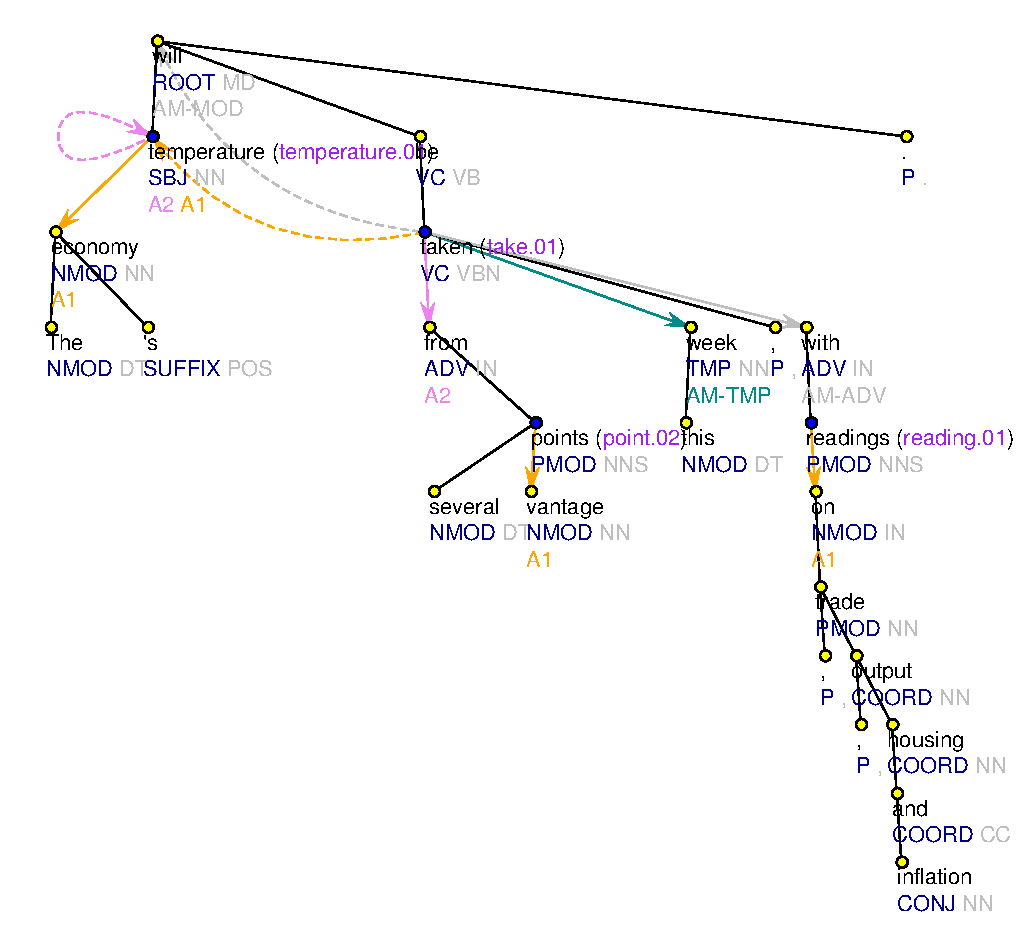
\includegraphics[height=4in,width=4.5in]{temperature-conll.eps}
$\begin{array}{cc}
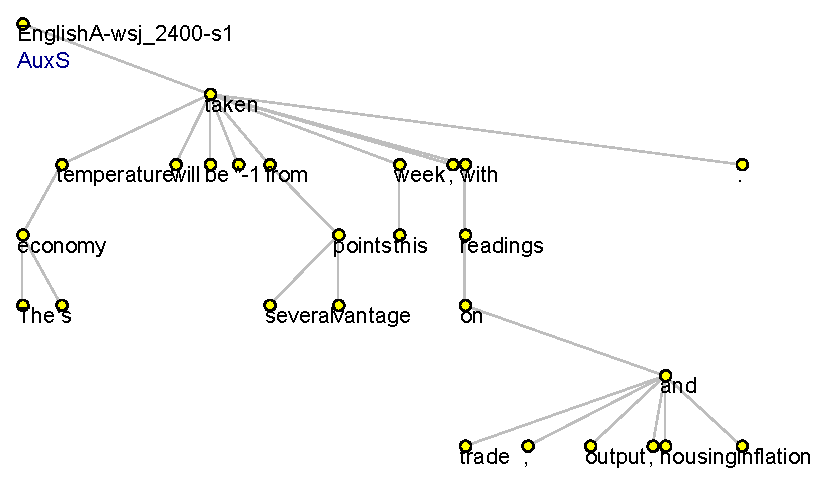
\includegraphics[height=2in,angle=270]{temperature-pedt-a.eps} & 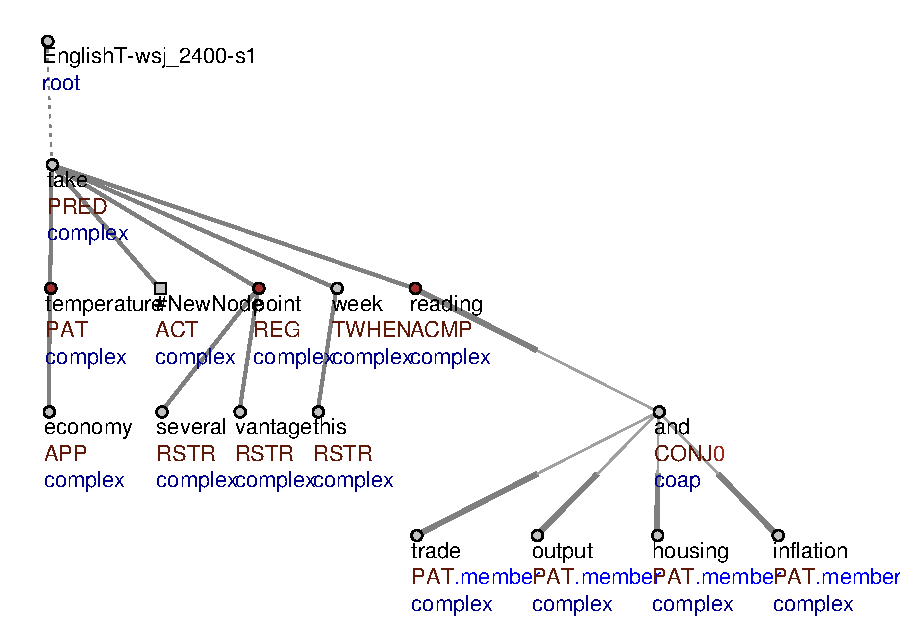
\includegraphics[height=2.75in,angle=270]{temperature-pedt-t.eps}
\end{array}$
\end{center}
\end{figure}

A comparison of both annotations is shown in Figure \ref{fig:tree-comp}\footnote{The tree images were created by the TrEd tree editor\\(\url{http://ufal.mff.cuni.cz/\~pajas/tred/}).}. It is apparent that the PEDT annotation contains more semantic information, because it also contains semantic dependencies of adjectives and adverbs, as well as more detailed structure when compared to the two-level structure of PropBank and NomBank. The semantic role labels, which adhere to the FGD, are also different from the numbered arguments of PropBank and NomBank, even though the PEDT valency lexicon EngVALLEX \citep{semecky06} is originally based on PropBank and NomBank frames. While most of the labels remain semantically constant across different predicates, the most widely ones are subject to \emph{shifting} with verbs, i.e. the first argument of any verb is always called \texttt{ACT} and the second one \texttt{PAT}, even if they do not denote the semantic roles of an actor and an affected object\footnote{Cf. a detailed description in the annotation guidelines at: \\ \url{http://ufal.mff.cuni.cz/\~cinkova/TR\_En.pdf}, pg. 36ff. and 107ff.}. Also the references are treated in a different way: Additional links are inserted into the otherwise tree structure to represent them.

It is however still possible to find some common grounds between the two sources --- both of them include labeled dependencies between noun and verbal predicates and their required or voluntary arguments. The Czech part of the CoNLL 2009 contest included the PDT data whose annotation schema is also based on the FGD and uses the same dependency concept; therefore, it is probably feasible to tweak a SRL system designed for the CoNLL annotation for use with the PEDT data, as long as it remains within the limits of finding arguments of noun and verb predicates. Full semantic dependency parsing would require more radical modifications.

\section{The CoNLL Corpus: Data Format and Statistics}\label{data-format}

Since we have described the annotation schema and sources of the CoNLL 2009\footnote{Since the concrete data format differs slightly from the 2008 version, we will now refer solely to the data sets used in this thesis.} corpus, we may now turn our attention to its technical implementation. The data is divided into three sets: \emph{training}, \emph{development} (tuning) and (final) \emph{evaluation} sentences. Each of them is included in a single text file, which contains all the plain text, morphological, syntactic and semantic information. Each line in every text file comprises all the knowledge about one token (i.e. word or punctuation sign), the individual inputs divided by tabs, forming columns. The purpose of each column is described in Table \ref{tab:st-columns}\footnote{Please see \url{http://ufal.mff.cuni.cz/conll2009-st/task-description.html} for further explanation.}. Different sentences are separated by empty lines.

\begin{table}[htbp]\footnotesize
\caption{The data columns of the CoNLL Shared Task corpus format}\label{tab:st-columns}
\begin{center}
\begin{tabular}{|r|l|l|}\hline
\bf No. & \bf Name & \bf Contents \\\hline
1 & ID & Number of the token in the sentence \\
2 & FORM & The word form as it appears in the original text \\
3 & LEMMA & Gold standard dictionary lemma of the word form \\
4 & PLEMMA & Automatically predicted lemma \\
5 & POS & Gold standard part-of-speech \\
6 & PPOS & Automatically predicted part-of-speech \\
7 & FEAT & \multirow{2}{*}{(Not used for English)} \\
8 & PFEAT & \\
9 & HEAD & ID of the syntactic head of this word (0 for root node; gold standard) \\
10 & PHEAD & Automatically predicted syntactic head ID \\
11 & DEPREL & Dependency relation label (gold standard) \\
12 & PDEPREL & Automatically predicted dependency relation label \\
13 & FILLPRED & Contains \texttt{Y}, if the word is a predicate \\
14 & PRED & The predicate name (lemma and sense number) \\
15+$i$ & APRED$i$ & Arguments of $i$-th predicate in the sentence \\\hline
\end{tabular}
\end{center}
\end{table}

\begin{figure}[htbp]
\caption{An example sentence from the CoNLL Shared Task Corpus}\label{fig:st-sample}
\begin{center}
\resizebox{\textwidth}{5cm}{
\begin{tabular}{llllllllllllllllllll}
1 & The & the & the & DT & DT & \_ & \_ & 2 & 2 & NMOD & NMOD & \_ & \_ & \_ & \_ & \_ & \_\\
2 & economy & economy & economy & NN & NN & \_ & \_ & 4 & 4 & NMOD & NMOD & \_ & \_ & A1 & \_ & \_ & \_\\
3 & 's & 's & 's & POS & POS & \_ & \_ & 2 & 2 & SUFFIX & SUFFIX & \_ & \_ & \_ & \_ & \_ & \_\\
4 & temperature & temperature & temperature & NN & NN & \_ & \_ & 5 & 5 & SBJ & SBJ & Y & temperature.01 & A2 & A1 & \_ & \_\\
5 & will & will & will & MD & MD & \_ & \_ & 0 & 0 & ROOT & ROOT & \_ & \_ & \_ & AM-MOD & \_ & \_\\
6 & be & be & be & VB & VB & \_ & \_ & 5 & 5 & VC & VC & \_ & \_ & \_ & \_ & \_ & \_\\
7 & taken & take & take & VBN & VBN & \_ & \_ & 6 & 6 & VC & VC & Y & take.01 & \_ & \_ & \_ & \_\\
8 & from & from & from & IN & IN & \_ & \_ & 7 & 7 & ADV & ADV & \_ & \_ & \_ & A2 & \_ & \_\\
9 & several & several & several & DT & DT & \_ & \_ & 11 & 11 & NMOD & NMOD & \_ & \_ & \_ & \_ & \_ & \_\\
10 & vantage & vantage & vantage & NN & NN & \_ & \_ & 11 & 11 & NMOD & NMOD & \_ & \_ & \_ & \_ & A1 & \_\\
11 & points & point & point & NNS & NNS & \_ & \_ & 8 & 8 & PMOD & PMOD & Y & point.02 & \_ & \_ & \_ & \_\\
12 & this & this & this & DT & DT & \_ & \_ & 13 & 13 & NMOD & NMOD & \_ & \_ & \_ & \_ & \_ & \_\\
13 & week & week & week & NN & NN & \_ & \_ & 7 & 7 & TMP & TMP & \_ & \_ & \_ & AM-TMP & \_ & \_\\
14 & , & , & , & , & , & \_ & \_ & 7 & 7 & P & P & \_ & \_ & \_ & \_ & \_ & \_\\
15 & with & with & with & IN & IN & \_ & \_ & 7 & 7 & ADV & ADV & \_ & \_ & \_ & AM-ADV & \_ & \_\\
16 & readings & reading & reading & NNS & NNS & \_ & \_ & 15 & 15 & PMOD & PMOD & Y & reading.01 & \_ & \_ & \_ & \_\\
17 & on & on & on & IN & IN & \_ & \_ & 16 & 16 & NMOD & NMOD & \_ & \_ & \_ & \_ & \_ & A1\\
18 & trade & trade & trade & NN & NN & \_ & \_ & 17 & 17 & PMOD & PMOD & \_ & \_ & \_ & \_ & \_ & \_\\
19 & , & , & , & , & , & \_ & \_ & 18 & 18 & P & P & \_ & \_ & \_ & \_ & \_ & \_\\
20 & output & output & output & NN & NN & \_ & \_ & 18 & 18 & COORD & COORD & \_ & \_ & \_ & \_ & \_ & \_\\
21 & , & , & , & , & , & \_ & \_ & 20 & 20 & P & P & \_ & \_ & \_ & \_ & \_ & \_\\
22 & housing & housing & housing & NN & NN & \_ & \_ & 20 & 20 & COORD & COORD & \_ & \_ & \_ & \_ & \_ & \_\\
23 & and & and & and & CC & CC & \_ & \_ & 22 & 22 & COORD & COORD & \_ & \_ & \_ & \_ & \_ & \_\\
24 & inflation & inflation & inflation & NN & NN & \_ & \_ & 23 & 23 & CONJ & CONJ & \_ & \_ & \_ & \_ & \_ & \_\\
25 & . & . & . & . & . & \_ & \_ & 5 & 5 & P & P & \_ & \_ & \_ & \_ & \_ & \_\\
\\
\end{tabular}
}
\end{center}
\end{figure}

It is apparent from Figure \ref{fig:st-sample} that the corpus data format is economic -- no data is repeated -- and easily human-readable. Manual analysis of corpus sentences is further simplified by the CoNLL 2009 Shared Task Extension for the TrEd tool\footnote{\url{http://ufal.mff.cuni.cz/\~pajas/tred/extensions/}}. On the other hand, the \texttt{APRED} columns and their different number for different sentences, as well as the fact that their order is only determined by the order of predicates in the sentence, clearly means that such a data format is not well suitable for usual machine learning classifiers, since they require a constant data structure for the whole set. We will discuss the data conversion further in Section \ref{conversion}.

\begin{table}[htbp]
\caption{Corpus size and coverage statistics for the CoNLL 2009 corpus used in this thesis}\label{tab:corpus-stats}
\begin{center}
\begin{tabular}{|c|rrrrrr|}\hline
  & \multirow{2}{*}{\bf Tokens} & \multirow{2}{*}{\bf Sentences} & \multicolumn{2}{c}{\bf Predicates} & \multicolumn{2}{c|}{\bf Coverage} \\
 & & & Unique & All & Unique & All \\\hline
Training & 958167 & 39279 & 9228 & 179014 & - & - \\
Development & 33368 & 1334 & 2151 & 6390 & 94.9 \% & 98.2 \% \\
Evaluation & 57676 & 2399 & 2610 & 10498 & 95.6 \% & 98.8 \% \\\hline
\end{tabular}
\end{center}
\end{table}

The CoNLL corpus covers virtually all of the original PTB texts, while the vast majority of the data is selected for training purposes. Table \ref{tab:corpus-stats} shows that most of the predicates and virtually all predicates with more than one occurrence in the development or evaluation set are covered by the training set, but a small group of unseen data will need to be treated separately. The average number of predicates per sentence is $4.55$ in the training data set. Therefore, if the system is set-up to classify the arguments of one predicate at a time (which is the only option with classic machine learning classifiers), the amount of data will multiply by that number. This means more training data instances and therefore possibly a higher classification precision; on the other hand, more computing resources will be needed to process such quantity.

%
%
\chapter{The Used Machine Learning Environment}\label{mlprocess}
%
%

In order to achieve an easy configurability of experiments needed for the SRL system setup and their fast parallel processing on multiple interconnected computers in a computing grid or cluster, we have developed a special software framework\footnote{\url{http://code.google.com/p/en-deep/}}. We have chosen to implement it in Java environment because of its portability, performance and simple debugging and maintenance with the help of integrated development tools. Our intention to use existing classifiers and other NLP tools in our system (see Section \ref{weka}) also spoke in favor of Java, for many of the freely available utilities feature a Java API\nomenclature{API}{Application Programming Interface}. We will now describe the basic concepts used by our system --- the decomposition of an experiment into subtasks (Section \ref{tasks}), their batch processing (Section \ref{expansions}) in parallel (Section \ref{parallel}) and the integration of existing third-party libraries (Section \ref{weka}).

\section{Splitting the Experiments into Subtasks}\label{tasks}

As we described already in Section \ref{problem}, the whole SRL process that is the subject of this thesis consists of several multiple subtasks. Having considered the pipeline approach to the system architecture and the implementation of multiple classifiers for different lemmas or senses (see Section \ref{related} for details), we realized that it will be profitable to divide the whole analysis into very simple and compact subtask and process some of them in parallel. It is apparent that for multiple classifiers or other operations on independent parts of the data, parallelization is feasible and speeds up the whole process, thus allowing more time-consuming computation. 

We have considered employing the GNU Make utility\footnote{\url{http://www.gnu.org/software/make/}}, but decided to create our own, more specific application, which would allow us to define our custom description of the task with simpler subtask specifications\footnote{This also includes the \emph{task expansions} described in Section \ref{expansions}.}, as well as running not only in multiple threads, but also in multiple processes running on different computers in a cluster. 

We also decided to implement all the possible tasks as functions within a single executable application in order to reduce the OS overhead for process creation. The intended implementation in Java offered a simple concept which makes this possible while still maintaining modularity and extensibility: Every subtask is defined as a Java class derived from the base class called \texttt{Task}. In order to enable configurability, the individual settings or parameters of all the subtasks are then represented as name-value pairs handled by their concrete implementations\footnote{It is of course possible that some tasks do not need any parameters, which is regarded as an empty list of parameters. Similarly, binary parameters are viewed as parameters with an empty value.}. We divided all the tasks implemented in our system into three groups for convenience: the classification, evaluation and data manipulation tasks.

Although it is possible to process many tasks in parallel, there will necessarily be dependencies among some of them --- one subtask requiring the output of another subtask as it input. The dependencies should further be handled in such a way that it is still possible to use multiple machines for the computation. We have chosen the only straightforward way to implement this, even if it poses a load on the interconnecting network: The inputs and outputs of all tasks are always saved to files. This further simplifies the description of the subtask dependencies -- it is possible to determine the necessary flow of the SRL process only by examining the names of input and output files of the individual tasks.

\begin{figure}
\caption{Subtask definition example}\label{fig:scenario}
\begin{center}
\begin{lstlisting}
# this is a commentary
task sttoarff; # id of the subtask
    algorithm: # used Java class
        en_deep.mlprocess.manipulation.StToArff; 
    params: lang_conf="st-en.conf", # its settings
        divide_senses, one_file,  # parameters with no value (binary)
        generate="Children, DepPath, HeadPos", # parameters
        cluster_file="clusters-plain.txt";     # with values set
    in: "train.txt"; # inputs listing
    out: "train.arff"; # outputs listing
end;
\end{lstlisting}
\end{center}
\end{figure}

This all yields a task description which consists of a Java class name, its parameters and a list of inputs and outputs, which also define its dependencies and prerequisites. The whole experiment is then a list of such (sub)tasks. We represent the descriptions in a simple configuration file called the \emph{scenario} (see Figure \ref{fig:scenario}), which is parsed and topologically sorted \citep{kahn62} to create a to-do list or \emph{plan}, used by the individual running processes (see Section \ref{parallel}) to retrieve the next subtasks that need to be computed: Each subtask description in the plan contains an indication whether all of its prerequisites have already been completed.

\section{Wildcards and Task Expansion}\label{expansions}

Since we planned on using multiple machine learning classifiers or other operations which run multiple times on different data sets, we needed to have some means of describing that the same subtask should run several times with different data. Therefore, we introduced simple wildcards into the description of the inputs and outputs of subtasks. An asterisk character (``*'') in a file name within the input or output specifications may stand for any string, thus forming a pattern. All the files from the current directory that match it are then transfered to the subtask definitions in the following two modes determined by the number of asterisks in the file name:
\begin{itemize}
    \item \emph{Expanding mode (``*'')}, which cause the subtask to \emph{expand} to multiple tasks, each taking one of the matching files. If there are multiple expanding mode patterns in the input specifications, only the corresponding ones, i.e. those where the ``*'' stands for the same string, are put together to create an expanded task (see Figure \ref{fig:expansion} for an example).
    \item \emph{Listing mode (``**'')}, which let the subtask take all the matching files as its input, or create multiple matching files on the output. The output expansions are left up to the individual impelementations of the subtasks.
\end{itemize}

\begin{figure}
\caption{Task expansion example}\label{fig:expansion}\footnotesize
\begin{center}
Note that \texttt{data-a.dat} is not combined with \texttt{setting-b.dat}.

\begin{tabular}{m{3cm} c m{4.1cm} c m{4.1cm}}
\textbf{Work directory:}\par data-a.dat \par data-b.dat \par setting-a.conf \par setting-b.conf &
+ & 
\textbf{Original Task:} \par \begin{lstlisting}
task sample;
# (...)
in: "data-*.dat", 
    "setting-*.dat";\end{lstlisting} &
$\rightarrow$ &
\textbf{Expanded tasks:} \par \begin{lstlisting}
task sample^\#^a;
# (...)
in: "data-a.dat", 
    "setting-a.dat";\end{lstlisting} \par \begin{lstlisting}
task sample^\#^b;
# (...)
in: "data-b.dat", 
    "setting-b.dat";\end{lstlisting}
\end{tabular}
\end{center}
\end{figure}

These basic patterns were then further improved to suit all the batch processing needs during our experiments, so that they now allow for further specification enclosed in vertical bar (``\textbar'') characters immediately following the asterisk. The detailed specifications are ignored when determining the subtask dependencies, which allows to select just a subset of multiple outputs produced by subtask $A$ as the input of subtask $B$, while the dependency $A\rightarrow B$ remains. We also included the possibility to expand a task using inputs from different sources whose file names do not match (in contrast to the situation shown in Figure \ref{fig:expansion}), which results in a cartesian product. Further, it is possible to combine the two pattern modes in a limited way (only one ``**''-pattern is allowed in conjunction with ``*''-patterns), where at first, the listing mode is applied and then the expanding mode to the results of the first step\footnote{This possibility should be further extended, so that it is applicable to a wider variety of situations.}.

The expansion of a task is also transferred to its dependencies, if they contain the expanding mode patterns in their input specifications. This is done already with the expansion of the prerequisite task, so that the individual computing processes (see Section \ref{parallel}) may start working on some of the expansions of the dependency even if other prerequisite expansions are not yet finished. However, the topological order of the whole plan is always preserved. 
 
An important feature of our experiment framework is also the possibility that the individual tasks assign further subtasks themselves, which then occupy the immediately following position in the experiment plan. Inner dependencies of all such subtasks must always then result in one single termination subtask, so that the outer dependencies are left untouched. This allows for further parallelization of such time-consuming operations as greedy feature selection (see Section \ref{featsel}).

\section{Running the Tasks in Parallel}\label{parallel}

As we already mentioned in the previous sections of this chapter, our whole experiment software is designed to run in several instances in parallel. The number of working threads, i.e. the level of maximum possible parallelization along with the maximum possible load on the CPUs and data flow, is determined by the user: The main executable may be launched in multiple copies on the same machine, as well as on different computers in a cluster. There is also a possibility to start multiple threads within one program instance, which simplifies the usage with multi-core machines.

The running threads are then completely independent of one another --- the only information exchange among them takes place in the plan file (see Section \ref{tasks}). The thread that started as the first one automatically parses the experiment scenario configuration file, if it does not find the plan file in the working directory. Consequently, all the working instances retrieve the pending subtasks from the plan file and remove the completed ones, while indicating that any depending subtasks are no longer blocked. The number of tasks retrieved at a time by one computing thread may be configured for the particular experiment based on the complexity of its subtask, so that program instances do not get blocked and the input and output load on the plan file is not excessive.

If an error occurs within one of the subtasks, all the subtasks not depending on it will continue to be processed, so that the user can correct the error and relaunch only a part of the original plan. The logging feature with configurable verbosity simplifies the debugging of the experiment setup.

\section{Integration of Third-Party Libraries}\label{weka}

There is a wide variety of freely available NLP tools, such as classifiers or data filters, on the Internet. We decided to profit from some of them, while still keeping our framework relatively independent. Therefore, the individual implementations of various subtasks in our system use the integrated tools, but the task descriptions, the scenario and plan file format and the mechanisms that launch them in the correct order are independent of any third-party tools\footnote{Google Collections (\url{http://code.google.com/p/google-collections/}) and Java-GetOpt (\url{http://www.urbanophile.com/\~arenn/hacking/getopt/}) are the only exceptions from this rule. They are invisible to the programmer who creates additional subtask algorithms, though.}. It is very simple to use additional Java libraries and programs with our system, since for each tool, only one wrapper Java class which defines the subtask and calls the particular tool with the correct parameters needs to be implemented.

We have chosen to integrate the Waikato Environment for Knowledge Analysis \citep[WEKA][]{garner95}\footnote{Version 3.7.1, \url{http://www.cs.waikato.ac.nz/~ml/weka/}}\nomenclature{WEKA}{Waikato Environment for Knowledge Analysis} with most of the subtasks our system, since it offers a very wide collection of classifiers, feature selection algorithms and data filters with a unified API and a transparent default data format --- the Attribute-Relation File Format (ARFF)\nomenclature{ARFF}{Attribute-Relation File Format}, which thus became the default format for our classification tasks.

As one of our classification subtasks uses the Integer Linear Programming technique (see \ref{post-inference}), we also included the LP\_Solve\footnote{Version 5.5, \url{http://lpsolve.sourceforge.net/}.} tool into our system. Although the program is written in the C++ programming language and called via a wrapper library using Java Native Interface (JNI)\nomenclature{JNI}{Java Native Interface}, which makes it less portable among different computer platforms, this problem is bound solely to the subtask that uses this utility.

%
%
\chapter{Machine Learning in Semantic Analysis}\label{ml-semantic}
%
%

After careful consideration of the various machine learning solutions available (most of which were already discussed in Chapter \ref{related}), we decided to use the traditional supervised classifiers, such as SVM or MaxEnt, in our SRL system due to their competitive performance and simple configuration. The inclusion of many different algorithms in one software package --- WEKA --- poses also an advantage of this choice. We will now describe the basic concepts of the classification algorithms we tested in our experiments. As we already mentioned in Section \ref{data-format}, the original data format of the used corpus is not well-suited for the operation of machine learning procedures. Therefore, we also include an account of the data conversion that was required for their proper function.

\section{Classifiers}\label{classifiers}

As we already pointed out in Chapters \ref{intro} and \ref{related}, the \emph{Maxim Entropy} (MaxEnt) models \citep[p. 219ff.]{jelinek97} are one of the most used techniques in many different NLP tasks \citep[p. 607f.]{manning00} including SRL \citep{jiang06,zhao09,che09,chen09}. This is possibly thanks to the fact that their base idea of finding a conditional probability distribution with a maximum entropy subject to given constraints, i.e. ``the most uniform model subject to our knowledge'' \citep[p. 41]{berger96} is very straightforward and effective. The basic form of the conditional probability model \citep{malouf02}, which predicts a probability of target event (such as semantic class) $y$ given a context $x$, looks as follows: 
\begin{equation}
q_\theta(y|x) = \frac{\exp(\theta^T f(y)}{\sum y'\in Y(x) \exp(\theta^T f(y'))}
\end{equation}
The function $f$ corresponds to an $N$-dimensional vector of features (see Section \ref{features}) and $\theta$ is the corresponding weight vector. $Y$ determines all the possible events given the context $x$. The weights of the model are then trained to satisfy the maximum entropy condition, which is equivalent to minimizing the relative entropy \citep[or Kullback-Leibler Divergence][p. 72]{manning00} of the model $q_\theta$ to the empirical distribution $p$ observed on the training data (expectation of the individual features' frequencies), or maximizing the log-likelihood:
\begin{equation}
\min_\theta D(p||q_\theta) = \sum_{y,x} p(y,x) \log\frac{p(y|x)}{q_\theta(y|x)} = \max_\theta L(\theta) = \sum_{y,x} p(y,x) \log q_\theta(y|x)
\end{equation}
The techniques of fitting the model to the training data usually involve an iterative approach to the zero gradient of the log-likelihood function.

Another widely used approach to classification is the Support Vector Machine \citep{boser92}. Its basic idea is representing the (training) data as points in $N+1$-dimensional space, whose coordinates are given by the function $\phi(x)$ of the features and by the value of the target event $y$, and trying to separate the different target events with a hyperplane that has the maximum margin (distance to the nearest point). If we assume that the target event $y$ has only two possible values $\{1,-1\}$\footnote{Most SVM libraries are, however, capable of solving a problem with multiple possible target classes, e.g. by using multiple SVMs, each predicting one of the classes.}, the hyperplanes that are parallel to the maximum margin separator and touch the nearest data points of both target classes (the \emph{support vectors}) are then described by the equations:
\begin{equation}
w^T x + b = 1\quad\mbox{and}\quad w^T x + b = -1
\end{equation}
Maximizing the distance $\frac{2}{||w||}$ leads to minimizing $||w||$ under the circumstances that the hyperplane fits the training data, which yields the following optimization problem \citep{hsu03}, given training examples $x_i,y_i;\ i = 1\dots p$:
\begin{equation}\label{eq:svm-primal}
\min_{w,b} \frac{1}{2}w^T w\quad\mbox{subject to}\quad y_i(w^T\phi(x_i) + b)\geq 1
\end{equation}
This may then be transformed using Lagrangian multipliers \citep{cristianini00}:
\begin{equation}
\min_{w,b} \max_{\alpha} \frac{1}{2}w^T w - \sum_{i=1}^p \alpha_i(y_i(w^T\phi(x_i) _ b) - 1)
\end{equation}
Now we may solve the equation using Quadratic Programming and get the solution $w = \sum_{i=1}^p \alpha_i y_i \phi(x_i)$, $\sum_{i=1}^p \alpha_i y_i = 0$, which finally results in the optimization problem:
\begin{equation}
\max_{\alpha} = \sum_{i=1}^p \alpha_i - \frac{1}{2}\sum_{i=1}^p y_i y_j \alpha_i \alpha_j (\phi(x_i)^T \phi(x_j))\quad\mbox{subject to}\quad \sum_{i=1}^p \alpha_i y_i = 0,\ \alpha_i = 0\ \forall i
\end{equation}
The $\phi(x_i)^T \phi(x_j)$ term is called the \emph{kernel} function, while the most usual kernels are linear ($x_i^T x_j$)\footnote{In the CoNLL 2009 contest, \citet{che09} describes using SVM with this type of kernel.} and radial ($\gamma x_i^T x_j + r)^d$). As in most real-life classification problems it is impossible to find a hyperplane that would separate both target event values for all training examples, a regularization \citep{neumaier98} term $\xi$ is introduced into the Equation \ref{eq:svm-primal}, which penalizes classification errors, transforming it to the following shape \citep{cortes95}:
\begin{equation}
\min_{w,b} \frac{1}{2}w^T w + C\sum_{i=1}^p \xi_i \quad\mbox{subject to}\quad y_i(w^T\phi(x_i) + b)\geq 1 - \xi_i
\end{equation}
The $C$ parameter is then interpreted as the penalty cost. There are several possible shapes of the regularization function, most common being $L_1$ ($\max(1-y_i w^T x_i, 0)$) and $L_2$ ($\max(1-y_i w^T x_i, 0)^2$) norms for support vector machines \citep{fan08}.

The Logistic Regression \citep{hosmer00}, another common classifier type, is a variant of a generalized linear regression model \citep{maccullagh91}. The following model form is used to predict the binary target event $y$ given a feature vector $x$ and a weight vector $\theta$ \citep{lee06}:
\begin{equation}
p(y = 1|x,\theta) = \frac{1}{1 + \exp(-\theta^T x)}
\end{equation}


\section{Data Conversion}\label{conversion}
% prevod z puv. formatu do formatu pro klasifikatory
% sent-id word-id
\section{Features}\label{features}
% popis vsech featur, vc. word clusteru
\section{Feature Selection Algorithms}\label{featsel}
% ruzne druhy rankingu, mRMR, mutual information etc.
% greedy forward

\chapter{Predicate Disambiguation}\label{pd}
\section{Observations on the Data}
% urceni nekolika skupin ruzne "slozitych" problemu, podle poctu vyznamu slova
\section{Selecting the Classifier Setting}\label{classifier-setting}
% vyber nejlepsiho nastaveni klasifikatoru na testovaci mnozine
\section{Applying Multiple Feature Selection Algorithms}
% ruzna feature selection pro ruzne "slozite" predikaty
\section{The Predicate Disambiguation System}
% celkova organizace systemu, vc. nejakeho schematu

\chapter{Argument Labelling}\label{ac}
\section{Different Argument Types}
% prisl. urceni a reference nezavisi na valencnim ramci, valencni argumenty ano
% test s jednim klasifikatorem na vsechna data
% oddeleni klasifikace prisl. urceni a valencnich argumentu
\section{Argument Selection vs. Argument Labelling}
% oddeleni identifikace a klasifikace vs. klasifikace rovnou
\section{Merging Rare Predicates}
% slucovani ridkych predikatu se shodnym valencnim ramcem <- nezapomenout na prohazování pos, když vypadalo chybne
\section{Post-Inference on Valency Arguments}\label{post-inference}
% omezeni na neopakovani se valencnich roli
% pokusy s primitivnim klasifikatorem, s LPSolve 
\section{Adverbial Modifiers Labelling}
% problemy s pameti, rozdeleni dat a slucovani klasifikace
\section{The Argument Selection System}
% celk. organizace

\chapter{The Whole Deep Analysis System}\label{setup}
\section{Overall Organization}
% napojeni pred. disambiguation a argument labelling
\section{The Performance}
% vysledky, analyza (vhodne featury apod., problemy)

\chapter{Conclusions}\label{conclusions}
\section{Comparison to CoNLL 2009 Shared Task Systems}
\section{Further Possibilities of Improvement}
\section{Application to Prague English Dependency Treebank}
% kratky teoreticky navrh

\cleardoublepage
\addcontentsline{toc}{chapter}{List of Abbreviations}
\printnomenclature[2cm]
\cleardoublepage
\bibliographystyle{plainnat}
\addcontentsline{toc}{chapter}{Bibliography}
\bibliography{dipl}

\end{document}
